\section{Robot}

\subsection{Objectif}
Le robot doit manipuler les microcapsules en effectuant des tâches de \textit{pick and place} depuis leur zone de stockage jusqu'aux réacteurs. Il doit également être capable de manipuler des plaques de microcapsules et de \og{}Para-dox\fg{}.

\subsection{Contraintes}
\begin{enumerate}
    \item Respect des limites de la \textit{glove box} pour éviter toute collision;
    \item Gestion de deux outils (pince et module d'aspiration) sans changement manuel;
\end{enumerate}

\subsection{Méthode de programmation}
La programmation est effectuée en deux parties :
\begin{itemize}
    \item Les programmes intégrés au robot gèrent les déplacements : \og{}PickAndPlaceVial\fg{}, \og{}TakePlate\fg{}, et \og{}GivePlate\fg{} ;
    \item Un programme externe en Python appelle les fonctions du robot et transmet les informations nécessaires via l'interface RTDE (cf. \autoref{subsection:CommunicationRobot}).
\end{itemize}

\subsection{Outils}
Les outils nécessaires pour réaliser la manipulation sont :
\begin{itemize}
    \item une pince pour saisir les \textit{well plate} et les plaques \og{}Para-dox\fg{};
    \item un module pour l'aspiration des microcapsules.
\end{itemize}
Une pointe a également été fabriquée, pour faciliter la programmation des différents repères nécessaires.

Pour ajouter les outils, il faut, pour chaque outil, connaître la position du TCP par rapport à la bride du robot, il faut également connaître son centre de masse et son poids.
Il existe sur le robot, un programme permettant de récupérer toutes les informations nécessaires. Les trois outils ont été implémentés grâce à ce programme.


\subsection{Sécurité}
\subsubsection*{Limites de sécurité}
Les robots d'Universal Robot permettent de configurer des plans de sécurité, qui ne seront pas franchissables par le TCP du robot. Dans ce cas, deux limites des sécurités sont nécessaires, une par porte de la \textit{glove box}.
Pour définir ces limites, il faut :
\begin{enumerate}
    \item Définir un point en mettant l'outil perpendiculaire au plan souhaité.
    \item Définir un plan de sécurité qui passe par ce point et qui sera normal à l'outil du robot.
    \item Définir la sécurité à mettre en place (Normal, réduit, les deux ou mode de déclenchement réduit). Dans notre cas, nous ne voulons pas que le TCP dépasse ces plans, le mode \og{}les deux\fg{} doit donc être appliqué.
\end{enumerate}

\subsection{Repères de travail}
Deux repères seront utilisés :
\begin{itemize}
    \item le repère de base qui sera utilisé pour déplacer les plaques;
    \item le repère \og{}repPickAndPlace\fg{} (\cf \autoref{img:plan_pickandplace}), sera utilisé pour le déplacement des microcapsules.
\end{itemize}
\begin{figure}[H]
    \centering
    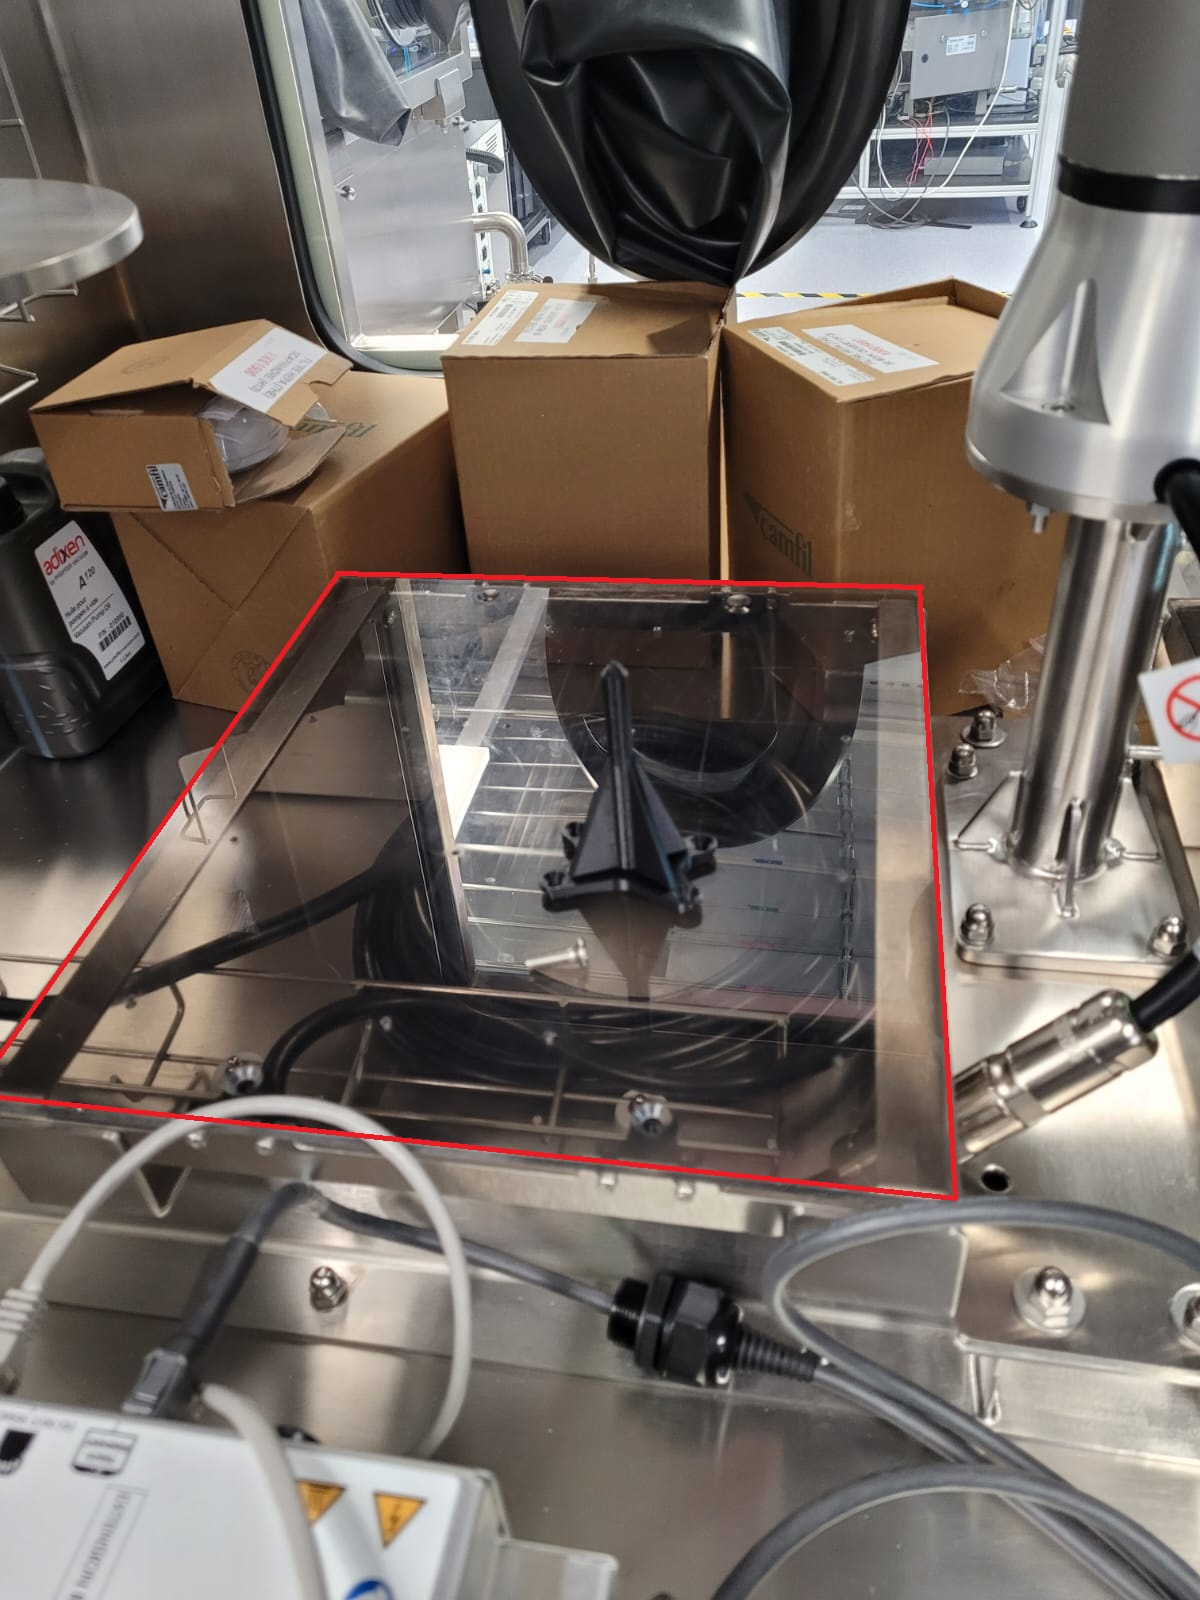
\includegraphics[width=\textwidth/2]{assets/figures/Hardware/plan/planPickAndPlace.jpeg}
    \caption{Position physique du plan \og{}repPickAndPlace\fg{}}
    \label{img:plan_pickandplace}
\end{figure}
\subsection{Communication avec le robot}\label{subsection:CommunicationRobot}
L'interface \textit{Real-Time Data Exchange} (RTDE) permet l'échange bidirectionnel en temps réel des données entre le robot et le système externe, facilitant ainsi le démarrage des programmes robot et la lecture/écriture des registres nécessaires.
